%% abtex2-modelo-slides.tex, v-1.0 gfabinhomat
%% Copyright 2012-<COPYRIGHT_YEAR> by abnTeX2 group at http://www.abntex.net.br/ 
%%
%% This work may be distributed and/or modified under the
%% conditions of the LaTeX Project Public License, either version 1.3
%% of this license or (at your option) any later version.
%% The latest version of this license is in
%%   http://www.latex-project.org/lppl.txt
%% and version 1.3 or later is part of all distributions of LaTeX
%% version 2005/12/01 or later.
%%
%% This work has the LPPL maintenance status `maintained'.
%% 
%% The Current Maintainer of this work is Fábio Rodrigues Silva, 
%% member of abnTeX2 team, led by Lauro César Araujo. 
%% Further information are available on 
%% http://www.abntex.net.br/
%%
%% This work consists of the files abntex2-modelo-slides.tex, 
%% abntex2-modelo-references.bib and abntex2-modelo-marca.pdf
%%
%% Modelo desenvolvido por Fábio Rodrigues Silva (gfabinhomat@gmail.com)
%% Mais informações podem ser obtidas no guia do usuário Beamer 
%% (http://linorg.usp.br/CTAN/macros/latex/contrib/beamer/doc/beameruserguide.pdf)
%% Informações rápidas podem ser acessadas em http://en.wikibooks.org/wiki/LaTeX/Presentations

\pdfminorversion=7

% Apresentações em widescreen. Outros valores possíveis: 1610, 149, 54, 43 e 32.
% Por padrão, as apresentações são no formato 4:3 (sem o aspectratio).
\documentclass[aspectratio=43]{beamer}	 	

\usetheme{PaloAlto}
\usecolortheme{spruce}
% Enconte mais temas e cores em http://www.hartwork.org/beamer-theme-matrix/ 
% Veja também http://deic.uab.es/~iblanes/beamer_gallery/index.html

\definecolor{ifprgreen}{RGB}{0,61,30}
\definecolor{ifprlightgreen}{RGB}{139,239,67}
\definecolor{ifprred}{RGB}{212,0,0}
\definecolor{sectiongreen}{RGB}{140,186,163}

% Customizações de Cores: fg significa cor do texto e bg é cor do fundo
%\setbeamercolor{normal text}{fg=black}
%\setbeamercolor{alerted text}{fg=red}
%\setbeamercolor{frametitle}{fg=black}
%\setbeamercolor{framesubtitle}{fg=black}
\setbeamercolor{block title}{bg=ifprgreen}		%Cor do título
%\setbeamercolor{block body}{bg=lightgray, fg=darkgray}	%Cor do texto (bg= fundo; fg=texto)
%\setbeamercolor{section in sidebar}{bg=ifprlightgreen, fg=black}
\setbeamercolor{itemize item}{fg=yellow,bg=black}
\setbeamercolor*{item}{fg=ifprgreen}
\setbeamercolor{section in toc}{fg=black}
\setbeamercolor{caption name}{fg=black}
\setbeamercolor{subsection in sidebar}{fg=white}
\setbeamercolor{subsection in sidebar shaded}{fg=sectiongreen}

\setbeamertemplate{caption}[numbered]

\makeatletter
\logo{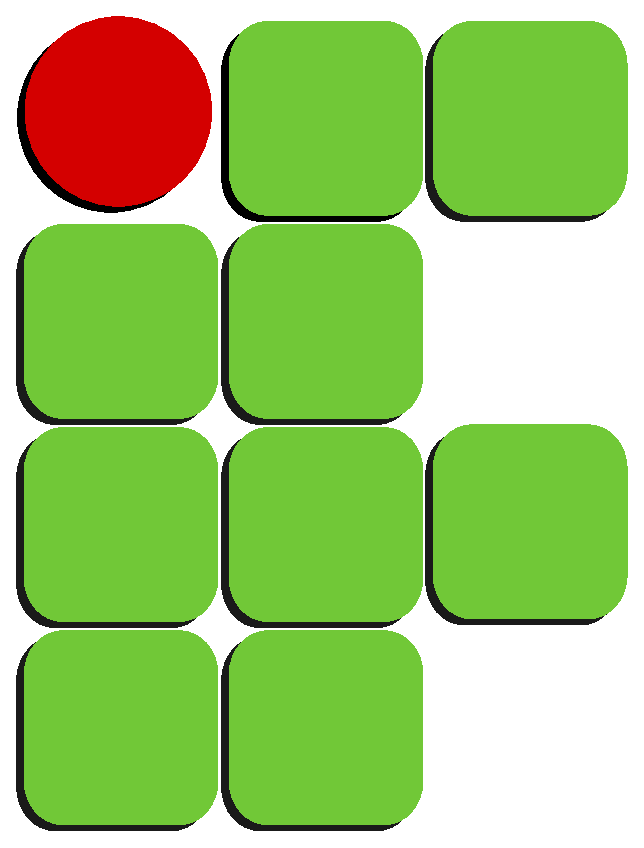
\includegraphics[height=.9\beamer@headheight]{logo_ifpr_shadow.eps}}
\makeatother

\makeatletter
\makeatletter
  \setbeamertemplate{sidebar \beamer@sidebarside}%{sidebar theme}
  {
    \beamer@tempdim=\beamer@sidebarwidth%
    \advance\beamer@tempdim by -6pt%
    \insertverticalnavigation{\beamer@sidebarwidth}%
    \vfill
    \ifx\beamer@sidebarside\beamer@lefttext%
    \else%
      \usebeamercolor{normal text}%
      \llap{\usebeamertemplate***{navigation symbols}\hskip0.1cm}%
      \vskip2pt%
    \fi%
}%
\makeatother

% ---
% PACOTES
% ---
\usepackage[alf]{abntex2cite}		% Citações padrão ABNT
\usepackage[brazil]{babel}		% Idioma do documento
\usepackage{color}			% Controle das cores
\usepackage{xcolor}			% Controle das cores
\usepackage[T1]{fontenc}		% Selecao de codigos de fonte.
\usepackage{graphicx}			% Inclusão de gráficos
\usepackage[utf8]{inputenc}		% Codificacao do documento (conversão automática dos acentos)
\usepackage{txfonts}			% Fontes virtuais
\usepackage{graphbox}
\usepackage{pgf}  
\usepackage{tikz}
\usepackage[default]{lato}
\usepackage{tabularx}
% ---

% --- Informações do documento ---
\title{Automatização de Mineração de Criptomoedas Com Distribuição Linux}
\author{Mateus Bittencourt Mercer \and Prof. Dr. Rodolfo Barriviera}
\institute{Instituto Federal do Paraná Campus Londrina}
\date{\today}
% ---

% ---
% Caminho das imagens
% ---
\graphicspath{{imagens/}}

% ----------------- INÍCIO DO DOCUMENTO --------------------------------------
\begin{document}

% ----------------- NOVO SLIDE --------------------------------
\begin{frame}
\titlepage
\end{frame}

% ----------------- NOVO SLIDE --------------------------------
\begin{frame}{Sumário}
\tableofcontents
\end{frame}

% ----------------- NOVO SLIDE --------------------------------
\section{Objetivos}

\begin{frame}{Objetivo Geral}

\noindent\makebox[\textwidth][c]{%
\begin{minipage}{10cm}
    Utilizar uma distribuição Linux para automatizar a configuração
    do software de criptomoeda.
\end{minipage}
}

\end{frame}

% ----------------- NOVO SLIDE --------------------------------
\begin{frame}{Objetivos Específicos}

\begin{itemize} 

    \item Buscar alternativas de personalização de uma distribuição
        Linux;

    \item Pesquisar diferentes criptomoedas e suas vantagens e
        desvantagens em diferentes hardwares;

    \item Encontrar as melhores alternativas de softwares em termos de
        praticidade e tempo;

    \item Comparar distribuições para a customização;

    \item Customizar uma distribuição;

    \item Fazer um comparativo da velocidade de instalação entre a
distribuição e uma instalação manual.

\end{itemize}
\end{frame}

% ----------------- NOVO SLIDE --------------------------------
\section{Introdução}
\begin{frame}
\frametitle{Introdução}
\framesubtitle{Contexto Geral das Criptomoedas}

%\begin{block}{Título}
% Este modelo foi preparado como uma aplicação do uso do pacote abnTeX2 com o Beamer.
%\end{block}
\begin{itemize}
    \item O \textbf{enfraquecimento do dólar} ajudou o advento das
        criptomoedas 

    \item As transferências \textbf{não dependem de uma instituição
        terceira}

    \item Em 2015, \textbf{mais de cem mil nós} estavam minerando
        Bitcoin 

    \item Existem \textbf{mais de 800 criptomoedas} cadastradas no site Coin
        Market Cap 

\end{itemize}

\end{frame}

% ----------------- NOVO SLIDE --------------------------------
\section[Desenvolvi\ldots]{Desenvolvimento}
\subsection{Mineração}

\begin{frame}
    \frametitle{Mineração}
    \framesubtitle{Recompensa e Prova de Trabalho}
    
    \begin{itemize}
        \item Quem minera recebe $N$ tokens pelo \textbf{trabalho} feito
            
        \item Minerar é \textbf{validar transações} no blockchain

        \item Os \textbf{nós na rede concorrem} para descobrir um
            número que quando juntado ao hash do bloco a ser minerado,
            o hash dessa junção possui $N$ zeros

        \item Os blocos são encadeados, \textbf{imutáveis} e
            \textbf{distribuídos}. ``corrente de blocos'' 

        \item \textbf{Prova de trabalho}
    \end{itemize}
\end{frame}


\begin{frame}
    \frametitle{Mineração}
    \framesubtitle{Visão Geral do Blockchain}
    
    \begin{figure}[H]
        \caption{\label{fig:blockchain-hash}Gráfico da visão geral
        do blockchain.}
        \begin{center}
            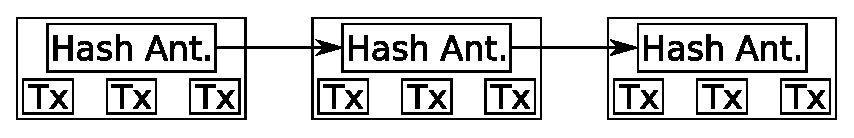
\includegraphics[width=1\linewidth]{blockchain-hash.eps}
        \end{center}
        Fonte: Adaptação de \cite{Nakamoto2008}
    \end{figure}
\end{frame}

% ----------------- NOVO SLIDE --------------------------------
\subsection{Transações}

\begin{frame}
    \frametitle{Transações}
    \framesubtitle{Usuários e Balanço}
    
    \begin{itemize}
        \item Usuários são \textbf{identificados com uma chave
            pública} e
            \textbf{acessam sua carteira com sua chave privada}

        \item No Bitcoin o \textbf{balanço é calculado pela lista de
            transações no blockchain}

    \end{itemize}
\end{frame}

\begin{frame}
    \frametitle{Transações}
    \framesubtitle{Transação de Bitcoin}
    
    \begin{figure}[H]
        \caption{\label{fig:exemplo-bitcoin}Exemplo de uma transferência
            com Bitcoin.}
        \begin{center}
            \includegraphics[width=.6\linewidth]{exemplo-bitcoin.pdf}
        \end{center}
        Fonte: O Autor.
    \end{figure}
\end{frame}

% ----------------- NOVO SLIDE --------------------------------
\subsection{Contratos Inteligentes}

\begin{frame}
    \frametitle{Contratos Inteligentes}
    \framesubtitle{Ethereum e Contratos Inteligentes}
    
    \begin{itemize}
        \item Contratos inteligentes são \textbf{programas que podem ser
            colocados no blockchain}

        \item São \textbf{imutáveis}, \textbf{distribuídos} e
            \textbf{não necessitam de uma instituição terceira para
            serem validados}

        \item Essa validação tem uma taxa, quanto mais rápida, mais
            cara, \textbf{quem recebe esta taxa são os mineradores}
    
    \end{itemize}
\end{frame}

% ----------------- NOVO SLIDE --------------------------------
\begin{frame}
    \frametitle{Contratos Inteligentes}
    \framesubtitle{Exemplo de Contrato Inteligente em Ethereum}
\begin{figure}[H]
    \caption{\label{fig:contratos-inteligentes}Exemplo de um contrato
    inteligente em Ethereum.}
    \begin{center}
        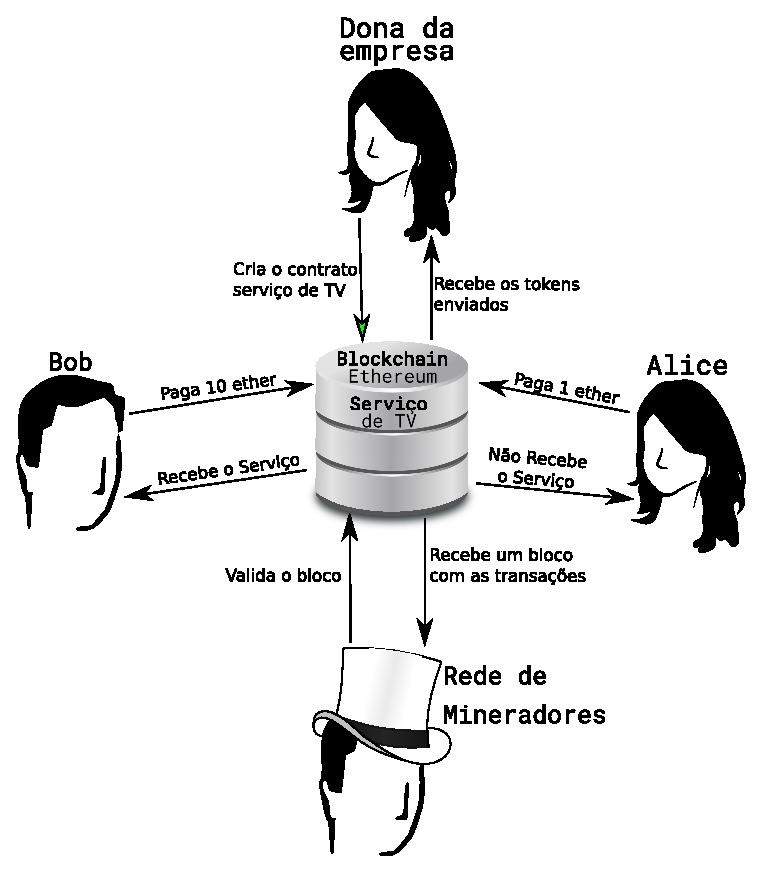
\includegraphics[width=.5\linewidth]{contratos-inteligentes.eps}
    \end{center}
    Fonte: O Autor.
\end{figure}

\end{frame}

% ----------------- NOVO SLIDE --------------------------------
\begin{frame}
    \frametitle{Contratos Inteligentes}
    \framesubtitle{Exemplo de Código de um Contrato Inteligente}
\begin{figure}[H]
    \begin{center}
        \includegraphics[width=.8\linewidth]{contrato-inteligente-tv.png}
    \end{center}
    Fonte: O Autor.
\end{figure}

\end{frame}

% ----------------- NOVO SLIDE --------------------------------
\subsection{Rigs de Mineração}

\begin{frame}
    \frametitle{Rigs de Mineração}
    \framesubtitle{Poder Computacional e Rigs de Mineração}

    \begin{itemize}
        \item Quanto \textbf{mais poder computacional, mais lucrativa} é a
            mineração (o algoritmo interfere diretamente)

        \item A medida utilizada para apresentar o desempenho de um
            rig de mineração é ``\textbf{hashes por segundo}'' $h/s$

    \end{itemize}
\end{frame}

% ----------------- NOVO SLIDE --------------------------------
\begin{frame}
    \frametitle{Rigs de Mineração}
    \framesubtitle{Rig de Mineração com 13 GPUs}

    \begin{figure}[H]
        \caption{\label{fig:rig_mineracao}Um rig de mineração com 13 GPUs
        NVidia 1060}
        \begin{center}
            \includegraphics[width=.3\linewidth]{rig_mineracao.png}
        \end{center}
        Fonte: \url{https://mining.bg/13-gpu-mining-rig-nvidia-1060-3gb-8/}
    \end{figure}
\end{frame}

% ----------------- NOVO SLIDE --------------------------------
\subsection{Distribuições Linux}
\begin{frame}
    \frametitle{Distribuições Linux}
    \framesubtitle{Contexto e Vantagens}

    \begin{itemize}
        \item Assim como as criptomoedas, a variedade de distribuições
            é extensa

        \item Uma distribuição Linux pode ser baseada em outra

        \item Seu uso possibilida \textbf{maior desempenho na
            mineração}
    
    \end{itemize}
\end{frame}

% ----------------- NOVO SLIDE --------------------------------
\section{Metodologia}
\begin{frame}
    \frametitle{Metodologia}
    \framesubtitle{Modelo de Prototipação Evolucionário}

    \begin{itemize}
        \item Planejamento

        \item Modelagem

        \item Validação

        \item Refinamento

    \end{itemize}
\end{frame}

% ----------------- NOVO SLIDE --------------------------------
\section{Resultados Parciais}

\begin{frame}
    \frametitle{Resultados Parciais}
    \framesubtitle{Distribuição Munix}

    \begin{itemize}
        \item Criação da \textbf{distribuição Munix} (\emph{Mining Unix}) 

        \item A distribuição já \textbf{detecta placas gráficas NVidia e
            minera Monero}

        \item A ferramenta archiso é utilizada para a criação
            \textbf{baseada no Arch Linux}

        \item O desempenho mostrou resultados positivos sobre a
            distribuição

    \end{itemize}
\end{frame}


% ----------------- NOVO SLIDE --------------------------------
\section{Considerações Finais}

\begin{frame}
    \frametitle{Considerações Finais}
    \framesubtitle{Melhoria da Distribuição e Trabalho}

    \begin{itemize}
        \item Dar suporte a novas criptomoedas

        \item Criar um instalador para a distribuição

        \item Estudar mais a fundo as criptomoedas e
            distribuições Linux

    \end{itemize}
\end{frame}

% ----------------- NOVO SLIDE --------------------------------

% \section{Referências}

% --- O comando \allowframebreaks ---
% Se o conteúdo não se encaixa em um quadro, a opção allowframebreaks instrui 
% beamer para quebrá-lo automaticamente entre dois ou mais quadros,
% mantendo o frametitle do primeiro quadro (dado como argumento) e acrescentando 
% um número romano ou algo parecido na continuação.

\begin{frame}<presentation:0>[noframenumbering]
\bibliography{referencias}
\end{frame}

% ----------------- FIM DO DOCUMENTO -----------------------------------------
\end{document}
